% ------------------------------------------------------------%
% 2020-12-05
% 2015-2020 - Emerson Ribeiro de Mello - mello@ifsc.edu.br
% ------------------------------------------------------------%
\documentclass[11pt]{ifscarticle}
\usepackage{ifscutils}
\usepackage[alf]{abntex2cite} % Citações padrão ABNT

\renewcommand*{\theusecase}{UC-\thesection.\arabic{usecase}}


\usepackage{lipsum}
\usepackage{pifont}
% Pacotes inseridos pelo usuário
\usepackage{setspace} % adicionado para espaçamento entre linhas


\AtBeginDocument{\thispagestyle{empty}}
\begin{document}
% ------------------------------------------------------------%
% Capa
% ------------------------------------------------------------%
\begin{titlepage}
\begin{center}
% Logotipo do IFSC

\includegraphics[scale=.7]{./figuras/ifsc-v}
\vspace{4cm}

\rule{\linewidth}{0.5pt} \\[6pt] 
\doublespacing
% Título
{\huge \bfseries Threads}\\  [4pt] 
%inserir materia acima

% Subtítulo
{\large Sistemas Operacionais - Laboratório 5}\\

\rule{\linewidth}{2pt}  \\[10pt]
\vspace{1cm}
\end{center}

\begin{minipage}{.9\linewidth}

% Nome do curso, disciplina e professor.
\begin{minipage}{0.18\textwidth}
\begin{flushleft} \large
\textbf{Curso:}\\
\textbf{Professor:}\\
\end{flushleft}
\end{minipage}~
\begin{minipage}{0.8\textwidth}
\begin{flushleft} \large
Engenharia de Telecomunicações\\
{Rogerio Pereira Junior}\\
\end{flushleft}
\end{minipage}
\end{minipage}
\vspace{3cm}

% Nome dos alunos
\begin{minipage}{.9\linewidth}
\begin{flushright}
\textbf{Aluno:}\\
Victor E. de L. Guerra\\
\end{flushright}
\end{minipage}
\vfill


% Coloque aqui a data
\begin{center}
31/03/2026
\end{center}

\end{titlepage}
%\pagestyle{firstpage}
% ------------------------------------------------------------%

% ------------------------------------------------------------%
% Para adicionar sumário
% ------------------------------------------------------------%
 \tableofcontents
 \clearpage
% ------------------------------------------------------------%


% ------------------------------------------------------------%
% Início do documento
% ------------------------------------------------------------%


\section{Objetivos}

    \begin{itemize}
        \item Compreender a criação e o ciclo de vida de Threads em C (Pthreads)
        \item Analisar o escalonamento, prioridades e estados de processos via Shell.
        \item Observar problemas de concorrência (Race Conditions).
        \item Praticar o controle de jobs (Foreground/Background) e sinais de terminação.
    \end{itemize}


\section{Experimento 1: Criando processos com fork() e analisando com ps}

    Este experimento tem como objetivo demonstrar a criação de processos em sistemas Unix utilizando a função \texttt{fork()}. Ao executar o programa, são gerados dois processos: o processo pai e o processo filho, cada um com seu identificador (PID). Em seguida, utilizou-se o comando \texttt{ps -f} para listar os processos em execução, permitindo identificar e diferenciar o processo pai do filho com base nos campos PID (Process ID) e PPID (Parent Process ID).

    \begin{figure}[h!] 
        \centering
        
\includegraphics[width=0.9\textwidth]{imagens/img-1.png}
        \caption{Output do terminal pelo comando \texttt{ps -gl}}
        \label{fig:figura1}
    \end{figure}

    Com base na saída que vemos no print acima, podemos afirmar que o processo pai é o processo com PID \textbf{24036} e o processo filho é o processo com PID \textbf{24037}. Podemos identificar isso por conta o PPID (Parent PID), confirmando que o processo \textbf{24037} é filho do processo \textbf{24036}

\section{Experimento 2: fork() + execve() e análise com ps}

    Este experimento tem como objetivo demonstrar a substituição de um processo utilizando a função \texttt{execve()}. Após a criação de um processo filho com \texttt{fork()}, o processo filho executa o programa \texttt{/bin/ls}, substituindo completamente seu código original. Enquanto isso, o processo pai continua sua execução normalmente. O comando \texttt{ps -gl} foi utilizado para observar o comportamento dos processos, evidenciando que o processo filho passa a executar um novo programa, mantendo, porém, o mesmo PID.

    \begin{figure}[h!] 
        \centering
        
\includegraphics[width=0.9\textwidth]{imagens/img-2.png}
        \caption{Output do terminal pelo comando \texttt{ps -gl}}
        \label{fig:figura2}
    \end{figure}

    A partir da saída do comando \texttt{ps -gl}, é possível identificar o processo que executou o comando \texttt{ls} observando a coluna \texttt{COMMAND}. No exemplo apresentado, o processo com PID \texttt{26125} aparece como \texttt{[ls] <defunct>}, indicando que ele executou o comando \texttt{ls}.

    Esse processo possui como PPID o valor \texttt{26124}, que corresponde ao processo pai (\texttt{./ex2}). Isso confirma que o processo filho foi responsável por executar o comando \texttt{ls} após a chamada de \texttt{execve()}.
    
    Após a execução de \texttt{execve()}, o código original do processo filho é completamente substituído pelo programa \texttt{/bin/ls}. Ou seja, nenhuma instrução do código original do filho é executada após essa chamada, pois a memória do processo é sobrescrita com o novo programa.
    
    O estado \texttt{<defunct>} indica que o processo filho já terminou sua execução, mas ainda não foi removido da tabela de processos, pois o processo pai ainda não realizou a chamada de \texttt{wait()} para coletar seu status de término.
    
    Comparando com a Parte 1, onde o processo filho executava apenas um trecho de código diferente do pai, nesta parte o comportamento é distinto: o filho deixa de executar o programa original e passa a executar um novo programa. Além disso, observa-se que o processo filho termina rapidamente após executar o \texttt{ls}, diferentemente da Parte 1, onde ambos permaneciam em execução devido ao uso de \texttt{sleep()}.


\section{Experimento 3: Criando múltiplos processos e visualizando com ps-
tree + grep}


    \begin{figure}[h!] 
        \centering
        
\includegraphics[width=0.9\textwidth]{imagens/img-3.png}
        \caption{Árvore de processos gerada pelo comando \texttt{pstree} no Experimento 3}
        \label{fig:figura3}
    \end{figure}
    
    A partir da execução do programa, foram criados múltiplos processos devido às chamadas sucessivas da função \texttt{fork()}. Como cada chamada de \texttt{fork()} duplica todos os processos existentes, o número total de processos cresce de forma exponencial.
    
    Neste experimento, o laço executa \texttt{fork()} três vezes. O número total de processos gerados pode ser calculado por $2^n$, onde $n$ é o número de chamadas de \texttt{fork()}. Assim, temos:
    
    \[
    2^3 = 8 \text{ processos}
    \]
    
    Portanto, ao final da execução, existem 8 processos no total (incluindo o processo original).
    
    Esse comportamento ocorre porque, a cada iteração, todos os processos existentes executam novamente o \texttt{fork()}, duplicando-se. Ou seja:
    \begin{itemize}
        \item Após o primeiro \texttt{fork()}: 2 processos
        \item Após o segundo \texttt{fork()}: 4 processos
        \item Após o terceiro \texttt{fork()}: 8 processos
    \end{itemize}
    
    A árvore de processos apresentada na Figura \ref{fig:figura3} ilustra essa estrutura hierárquica, onde cada processo gera novos processos filhos.
    
    Uma representação simplificada da árvore de processos é:
    
    
    \begin{verbatim}
        ex3
        |-- ex3
        |   |-- ex3
        |   |   |-- ex3
        |   |   `-- ex3
        |   `-- ex3
        |       |-- ex3
        |       `-- ex3
    \end{verbatim}


\section{Experimento 4: Quantidade de Processos e Saídas na Tela}

    O objetivo deste experimento é compreender como múltiplas chamadas da função \texttt{fork()} impactam a quantidade de processos criados e a saída exibida no terminal.
    
    \subsection{Código 1}
    
    Sem executar o código, observa-se que há duas chamadas de \texttt{fork()}. Como cada chamada duplica os processos existentes, o número total de processos será:
    
    \[
    2^2 = 4 \text{ processos}
    \]
    
    Portanto, a mensagem \texttt{"Oi"} será exibida 4 vezes.
    
    A árvore de processos pode ser representada como:
    
    \begin{verbatim}
    P
    |-- P1
    |   `-- P3
    `-- P2
    \end{verbatim}
    
    Após a execução, foi possível confirmar que a saída corresponde ao esperado, com a mensagem sendo exibida quatro vezes. Isso ocorre porque cada processo executa o \texttt{printf()} de forma independente.

    \begin{figure}[h!] 
        \centering
        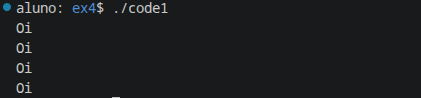
\includegraphics[width=0.9\textwidth]{imagens/img-4_1.png}
        \caption{Execução do Código 1}
        \label{fig:figura4_1}
    \end{figure}
    
    \subsection{Código 2}
    
    Neste caso, há três chamadas de \texttt{fork()}, resultando em:
    
    \[
    2^3 = 8 \text{ processos}
    \]
    
    Assim, a mensagem \texttt{"Oi"} será exibida 8 vezes.
    
    A árvore de processos pode ser representada como:
    
    \begin{verbatim}
    P
    |-- P1
    |   |-- P3
    |   |   |-- P7
    |   |   `-- P8
    |   `-- P4
    |       |-- P9
    |       `-- P10
    `-- P2
        |-- P5
        |   |-- P11
        |   `-- P12
        `-- P6
            |-- P13
            `-- P14
    \end{verbatim}
    
    Após a execução, o resultado confirmou a previsão, com a mensagem sendo exibida oito vezes.
    
    O crescimento do número de processos é exponencial, pois cada chamada de \texttt{fork()} duplica todos os processos existentes naquele momento. Assim, o total de processos segue a relação $2^n$, onde $n$ é o número de chamadas de \texttt{fork()}.

    \begin{figure}[h!]
        \centering
        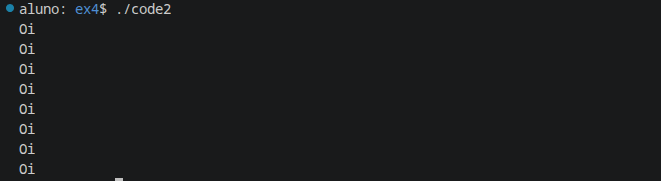
\includegraphics[width=0.9\textwidth]{imagens/img-4_2.png}
        \caption{Execução do Código 2}
        \label{fig:figura4_2}
    \end{figure}


\section{Experimento 5: Sincronização com wait()}

    O objetivo deste experimento é demonstrar a importância da chamada de sistema \texttt{wait()} para a sincronização entre processos pai e filho, evitando o surgimento de processos zumbis e garantindo a ordem de execução.

    O programa cria um processo filho que executa uma ``tarefa pesada'' (simulada com \texttt{sleep(5)}) e encerra com status 42. O processo pai utiliza \texttt{wait(\&status)} para aguardar o término do filho antes de prosseguir.

    \begin{figure}[h!]
        \centering
        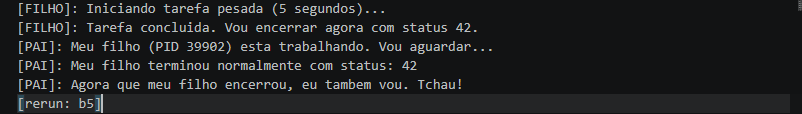
\includegraphics[width=0.9\textwidth]{imagens/img-5_1.png}
        \caption{Execução do Experimento 5 com \texttt{wait()} ativo}
        \label{fig:figura5}
    \end{figure}

    \begin{figure}[h!]
        \centering
        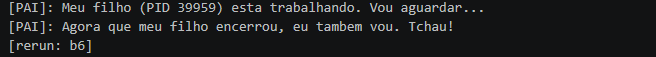
\includegraphics[width=0.9\textwidth]{imagens/IMG-5_2.png}
        \caption{Execução do Experimento 5 sem \texttt{wait()} (linha comentada)}
        \label{fig:figura5_sem_wait}
    \end{figure}

    \subsection{Questões para o Relatório}

    \textbf{1. No experimento com o \texttt{wait()} ativo, quem imprime a última mensagem no terminal? Por quê?}

    Com o \texttt{wait()} ativo, o processo pai imprime a última mensagem no terminal. Isso ocorre porque a chamada \texttt{wait(\&status)} bloqueia o processo pai até que o filho termine sua execução. Assim, a sequência é: o filho inicia, trabalha por 5 segundos, imprime sua mensagem de conclusão e encerra com \texttt{exit(42)}. Somente após isso, o pai retoma a execução, verifica o status do filho e imprime suas mensagens finais.

    \textbf{2. Quando você comentou o \texttt{wait()}, o que aconteceu com a ordem das mensagens? O pai esperou o filho?}

    Sem o \texttt{wait()}, o pai \textbf{não} esperou o filho. O processo pai continuou sua execução imediatamente após o \texttt{fork()}, imprimindo suas mensagens e encerrando antes mesmo do filho completar a tarefa de 5 segundos. Isso fez com que as mensagens do pai aparecessem primeiro, e as mensagens do filho aparecessem depois (ou nem aparecessem, dependendo do momento em que o pai encerrou). A ordem das mensagens ficou invertida em relação ao cenário com \texttt{wait()}.

    \textbf{3. O que são as macros \texttt{WIFEXITED} e \texttt{WEXITSTATUS}? Para que servem?}

    \begin{itemize}
        \item \texttt{WIFEXITED(status)}: é uma macro que retorna verdadeiro (não-zero) se o processo filho terminou normalmente, ou seja, por meio de uma chamada a \texttt{exit()} ou por retorno da função \texttt{main()}. Serve para verificar se o filho não foi encerrado por um sinal.
        \item \texttt{WEXITSTATUS(status)}: é uma macro que extrai o código de saída do processo filho (o valor passado para \texttt{exit()}). No caso deste experimento, retorna o valor 42, que foi o status de saída definido pelo filho.
    \end{itemize}

    \textbf{4. Explique por que o \texttt{wait()} é fundamental para evitar que o sistema fique cheio de processos ``zumbis''.}

    Quando um processo filho termina, ele entra no estado \textit{zombie} (zumbi): o processo já encerrou sua execução, mas sua entrada na tabela de processos ainda existe, aguardando que o pai colete seu status de término. A chamada \texttt{wait()} é o mecanismo pelo qual o pai coleta esse status, permitindo que o kernel remova definitivamente a entrada do filho da tabela de processos. Sem o \texttt{wait()}, os processos filhos encerrados permanecem como zumbis indefinidamente, consumindo entradas na tabela de processos do sistema. Se muitos processos zumbis se acumularem, o sistema pode esgotar o número máximo de processos permitidos, impedindo a criação de novos processos.


\section{Experimento 6: A Primeira Thread (Simples)}

    Este experimento demonstra a criação de uma thread simples utilizando a biblioteca Pthreads. O programa cria uma thread que imprime mensagens periodicamente, enquanto a thread principal aguarda com \texttt{pthread\_join()}.

    Utilizou-se o comando \texttt{ps -eL | grep exp01} para visualizar as threads do processo, onde a flag \texttt{-L} exibe os LWPs (\textit{Light Weight Processes}), que correspondem às threads no Linux. Também foi utilizado o comando \texttt{lsof -p [PID]} para listar os arquivos abertos pelo processo.

    \begin{figure}[h!]
        \centering
        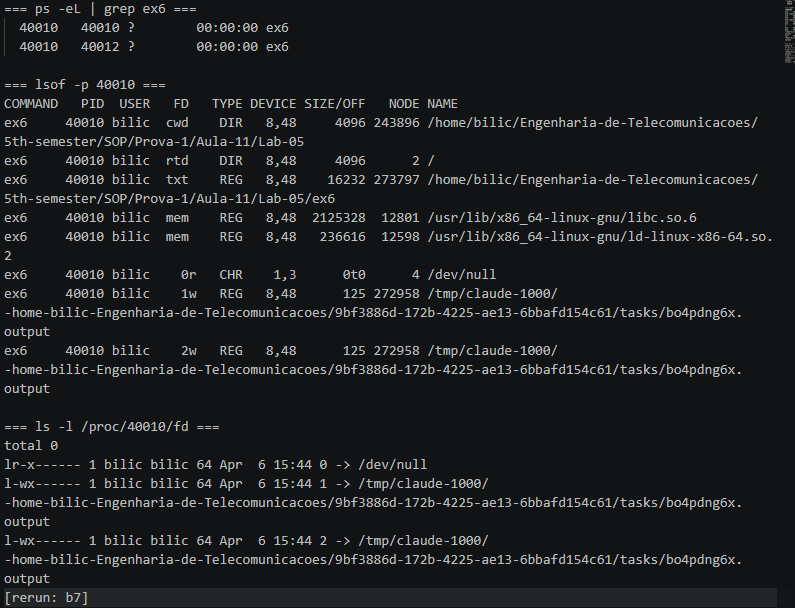
\includegraphics[width=0.9\textwidth]{imagens/IMG-6.png}
        \caption{Saída dos comandos \texttt{ps -eL | grep exp01} e \texttt{lsof -p [PID]}}
        \label{fig:figura6}
    \end{figure}

    Na saída do \texttt{ps -eL}, é possível observar que o processo possui dois LWPs (threads): a thread principal e a thread criada por \texttt{pthread\_create()}. Ambas compartilham o mesmo PID, mas possuem LWPs distintos, confirmando que threads existem dentro do mesmo espaço de endereçamento do processo.

    Na saída do \texttt{lsof}, observam-se os descritores de arquivo padrão (stdin, stdout, stderr) e os arquivos de bibliotecas compartilhadas carregadas pelo processo, como a \texttt{libpthread.so}.


\section{Experimento 7: O Contador de Threads}

    Neste experimento, foram criadas 4 threads com tempos de vida distintos (30s, 60s, 90s e 120s). O objetivo é observar o comportamento das threads ao longo do tempo utilizando o \texttt{htop}.

    \subsection{Respostas}

    \textbf{1. Descreva o que acontece no htop a cada intervalo de 30 segundos. As linhas desaparecem ou mudam de cor?}

    A cada intervalo de 30 segundos, uma thread finaliza e sua linha desaparece do \texttt{htop}:
    \begin{itemize}
        \item Aos 30s: a Thread 1 encerra e sua linha desaparece, restando 4 linhas (processo pai + 3 threads).
        \item Aos 60s: a Thread 2 encerra, restando 3 linhas.
        \item Aos 90s: a Thread 3 encerra, restando 2 linhas.
        \item Aos 120s: a Thread 4 encerra, e logo em seguida o processo principal também finaliza.
    \end{itemize}

    \textbf{2. No htop, as threads possuem o mesmo PID (Process ID) do processo pai?}

    Sim. No \texttt{htop}, todas as threads possuem o mesmo PID do processo pai. Isso ocorre porque threads compartilham o mesmo espaço de endereçamento e pertencem ao mesmo processo. O que as diferencia é o TID (\textit{Thread ID}) ou LWP, que é um identificador único atribuído pelo kernel a cada thread.

    \textbf{3. Por que o processo principal (pai) só termina após a última thread (de 120s) finalizar?}

    Porque o programa utiliza \texttt{pthread\_join()} para cada uma das 4 threads. A função \texttt{pthread\_join()} é bloqueante: ela faz com que a thread chamadora (neste caso, a thread principal) aguarde até que a thread especificada termine. Como o \texttt{join} é chamado sequencialmente para todas as threads, o processo principal só continua após a última thread (120s) encerrar.

    \textbf{4. Se você fechar o programa com Ctrl+C, o que acontece com as threads que ainda estavam rodando?}

    Ao pressionar \texttt{Ctrl+C}, o sinal \texttt{SIGINT} é enviado para o processo inteiro. Como todas as threads compartilham o mesmo processo, todas são encerradas imediatamente junto com o processo principal. Diferentemente de processos filhos criados com \texttt{fork()}, as threads não possuem existência independente do processo pai --- quando o processo morre, todas as suas threads morrem junto.


\section{Experimento 8: Concorrência e Race Condition}

    Neste experimento, duas threads incrementam simultaneamente uma variável global \texttt{contador} 1 milhão de vezes cada. O valor esperado ao final seria 2.000.000, mas devido à \textit{race condition}, o valor obtido é frequentemente menor.

    \begin{figure}[h!]
        \centering
        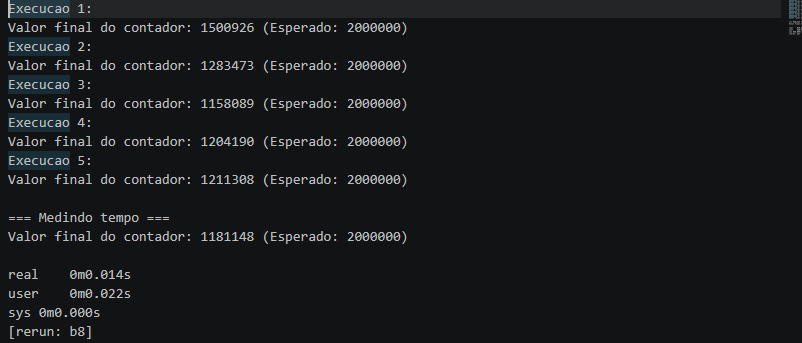
\includegraphics[width=0.9\textwidth]{imagens/IMG-8.png}
        \caption{Múltiplas execuções mostrando valores inconsistentes do contador}
        \label{fig:figura8}
    \end{figure}

    \textbf{O resultado muda? Por quê?}

    Sim, o resultado muda a cada execução. Isso ocorre devido a uma \textit{race condition} (condição de corrida). A operação \texttt{contador++} não é atômica --- ela é composta por três etapas: (1) ler o valor atual de \texttt{contador} da memória para um registrador, (2) incrementar o valor no registrador e (3) escrever o novo valor de volta na memória.

    Quando duas threads executam essas etapas simultaneamente, pode ocorrer a seguinte situação:
    \begin{enumerate}
        \item Thread A lê \texttt{contador} = 100
        \item Thread B lê \texttt{contador} = 100 (antes de A escrever)
        \item Thread A escreve \texttt{contador} = 101
        \item Thread B escreve \texttt{contador} = 101 (sobrescrevendo, perdendo um incremento)
    \end{enumerate}

    Esse problema é chamado de \textit{race condition} porque o resultado depende da ordem (``corrida'') em que as threads acessam a região crítica. Para resolver, seria necessário utilizar mecanismos de exclusão mútua, como \texttt{pthread\_mutex\_lock()} e \texttt{pthread\_mutex\_unlock()}, garantindo que apenas uma thread acesse a variável por vez.

    O comando \texttt{time ./programa} mostra que o tempo de execução é bastante curto (na ordem de milissegundos), o que confirma que ambas as threads executam em paralelo nos núcleos do processador.


\section{Experimento 9: Monitoramento de Longa Duração}

    Este experimento cria três threads com comportamentos distintos: duas threads CPU-intensivas (que executam cálculos matemáticos em laço infinito) e uma thread de I/O (que imprime mensagens periodicamente com \texttt{sleep(1)}).

    No \texttt{htop}, é possível observar que as duas threads CPU-intensivas consomem aproximadamente 100\% de um núcleo cada, enquanto a thread de I/O permanece com uso de CPU próximo de 0\%, pois passa a maior parte do tempo dormindo (\texttt{sleep}).

    O comando \texttt{renice} foi utilizado para alterar a prioridade (\textit{nice value}) do processo enquanto ele estava em execução. Por exemplo, \texttt{renice +10 -p [PID]} reduz a prioridade do processo, fazendo com que o escalonador do kernel dê menos tempo de CPU a ele em relação a outros processos. Isso demonstra como o sistema operacional permite o ajuste dinâmico de prioridades para gerenciar a alocação de recursos.


\section{Experimento 10: Simulação de Servidor Web}

    Neste experimento, simula-se um servidor web com 5 threads \textit{workers}, cada uma aguardando e processando ``requisições'' simuladas com tempos aleatórios.

    Para colocar o servidor em background, utilizou-se \texttt{Ctrl+Z} (que envia o sinal \texttt{SIGTSTP}, suspendendo o processo) seguido do comando \texttt{bg} (que retoma a execução do processo em segundo plano).

    Em seguida, utilizou-se \texttt{kill -9 [PID]} para enviar o sinal \texttt{SIGKILL} ao processo, encerrando-o forçadamente. Este sinal não pode ser capturado ou ignorado pelo processo, garantindo sua terminação imediata.

    \begin{figure}[h!]
        \centering
        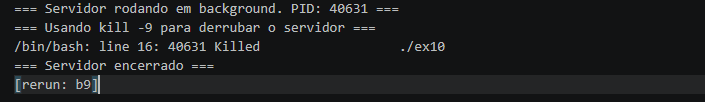
\includegraphics[width=0.9\textwidth]{imagens/IMG-10.png}
        \caption{Execução do servidor em background e encerramento com \texttt{kill -9}}
        \label{fig:figura10}
    \end{figure}

    Quando o \texttt{kill -9} é executado, o processo inteiro é encerrado, incluindo todas as 5 threads \textit{workers}. Como as threads compartilham o mesmo espaço de processo, não é possível matar o processo sem encerrar todas as suas threads. Esse comportamento difere de processos filhos criados com \texttt{fork()}, que possuem existência independente e continuariam em execução mesmo que o processo pai fosse encerrado.


\section{Desafio Final: Análise Teórica de Modelos de Threads}

    Nesta seção, analisa-se o comportamento do código proposto sob dois modelos de mapeamento de threads: \textbf{N:1} (Muitos para Um) e \textbf{1:1} (Um para Um).

    \subsection{A) Diagramas de Execução}

    \textbf{Modelo 1:1 (Um para Um):}

    No modelo 1:1, cada thread de usuário é mapeada diretamente para uma thread do kernel. Assim, quando uma thread executa \texttt{sleep()}, apenas ela é bloqueada, e as demais continuam executando.

    \begin{verbatim}
Tempo:  0s        1s        10s       11s       21s
        |---------|---------|---------|---------|---------|
main:   [cria tA, tB][sleep(1)][join tA][join tB][sleep(1)][cria tC][join tC]
tA:     [----sleep(10)----][print][exit]
tB:     [----sleep(10)----][print][exit]
tC:                                              [--sleep(10)--][print][exit]
    \end{verbatim}

    Neste modelo, tA e tB executam em paralelo. Ambas iniciam o \texttt{sleep(10)} quase simultaneamente e terminam aos ~10s. Após o \texttt{join} de ambas e o \texttt{sleep(1)} do main, tC é criada e roda por mais 10s.

    \textbf{Modelo N:1 (Muitos para Um):}

    No modelo N:1, todas as threads de usuário são mapeadas para uma única thread do kernel. Uma syscall bloqueante (\texttt{sleep}) bloqueia o processo inteiro.

    \begin{verbatim}
Tempo:  0s        10s       20s       21s       31s
        |---------|---------|---------|---------|---------|
main:   [cria tA,tB]            ...espera...
tA:     [---sleep(10)---][print][exit]
tB:                      [---sleep(10)---][print][exit]
main:                                    [sleep(1)][cria tC]
tC:                                                [---sleep(10)---][print][exit]
    \end{verbatim}

    Neste modelo, quando tA executa \texttt{sleep(10)}, o processo inteiro é bloqueado por 10 segundos. Somente após tA terminar, tB pode executar seu \texttt{sleep(10)}, bloqueando novamente por mais 10s. O mesmo ocorre com tC.

    \subsection{B) Durações Aproximadas}

    \begin{itemize}
        \item \textbf{Modelo 1:1:} Tempo total $\approx$ 22 segundos. As threads tA e tB executam em paralelo (~10s), seguidas de \texttt{sleep(1)} do main (~1s) e tC (~10s), mais o \texttt{sleep(1)} do main antes do join de tC, totalizando aproximadamente $10 + 1 + 1 + 10 \approx 22$s.
        \item \textbf{Modelo N:1:} Tempo total $\approx$ 32 segundos. As threads executam sequencialmente: tA (~10s) + tB (~10s) + \texttt{sleep(1)} do main + tC (~10s) + \texttt{sleep(1)} do main, totalizando aproximadamente $10 + 10 + 1 + 10 + 1 \approx 32$s.
    \end{itemize}

    \subsection{C) Saída do Programa}

    A saída do programa é a mesma em ambos os modelos:

    \begin{verbatim}
x: 1, y: 1
x: 1, y: 2
x: 1, y: 3
    \end{verbatim}

    \textbf{Justificativa:}

    \begin{itemize}
        \item A variável \texttt{x} é \textbf{local} à função \texttt{threadBody()}, portanto cada thread possui sua própria cópia de \texttt{x}. Em cada chamada, \texttt{x} é inicializada com 0 e incrementada para 1. Por isso, \texttt{x} sempre vale 1 na saída.
        \item A variável \texttt{y} é \textbf{global}, compartilhada entre todas as threads. Cada thread incrementa \texttt{y} com \texttt{++y}. Como as threads executam sequencialmente em ambos os modelos (no N:1 por bloqueio, no 1:1 porque tA e tB terminam antes de tC começar, e o \texttt{join} garante a ordem), os incrementos ocorrem de forma ordenada: a primeira thread imprime \texttt{y=1}, a segunda \texttt{y=2} e a terceira \texttt{y=3}.
    \end{itemize}

    A saída não difere entre os modelos porque, embora a ordem de execução temporal seja diferente, o efeito sobre as variáveis é o mesmo: cada thread incrementa \texttt{y} uma vez, e o mecanismo de \texttt{join} garante que o main aguarde o término de cada thread antes de prosseguir.


\end{document}